\documentclass[tikz,border=4pt]{standalone}
\usepackage{ctex}\usepackage{amsmath}
\usetikzlibrary{arrows.meta}
\begin{document}
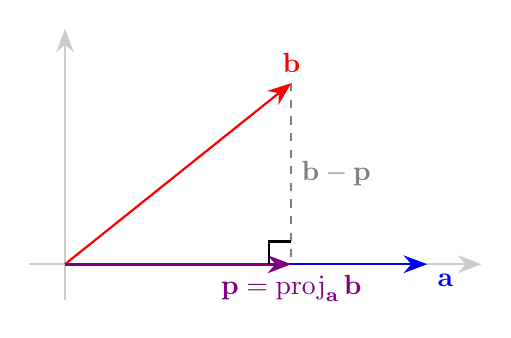
\begin{tikzpicture}[scale=1.15,>={Stealth[length=3mm]},thick]
  \draw[->,gray!40](-0.4,0)--(4.6,0);\draw[->,gray!40](0,-0.4)--(0,2.6);
  \draw[->,blue](0,0)--(4,0) node[below right]{$\mathbf{a}$};
  \draw[->,red](0,0)--(2.5,2) node[above]{$\mathbf{b}$};
  \draw[->,violet,very thick](0,0)--(2.5,0) node[below]{$\mathbf{p}=\operatorname{proj}_{\mathbf{a}}\mathbf{b}$};
  \draw[dashed,gray](2.5,2)--(2.5,0) node[midway,right]{$\mathbf{b}-\mathbf{p}$};
  \draw (2.25,0)--(2.25,0.25)--(2.5,0.25);
\end{tikzpicture}
\end{document}
